\documentclass[]{AVSSimReportMemo}
\usepackage{AVS}

\newcommand{\ModuleName}{hillPoint}
\newcommand{\subject}{Guidance Module for Hill Frame Pointing}
\newcommand{\status}{Initial Version}
\newcommand{\preparer}{M. Cols}
\newcommand{\summary}{Generate the attitude reference to perform a constant pointing towards a Hill frame orbit axis}


\begin{document}

\makeCover


%
%	enter the revision documentation here
%	to add more lines, copy the table entry and the \hline, and paste after the current entry.
%
\pagestyle{empty}
{\renewcommand{\arraystretch}{2}
\noindent
\begin{longtable}{|p{0.5in}|p{4.5in}|p{1.14in}|}
\hline
{\bfseries Rev}: & {\bfseries Change Description} & {\bfseries By} \\
\hline
Draft & initial copy & M. Cols \\
\hline

\end{longtable}
}

\newpage
\setcounter{page}{1}
\pagestyle{fancy}

\tableofcontents
~\\ \hrule ~\\

\begin{figure}[htb]
	\centerline{
	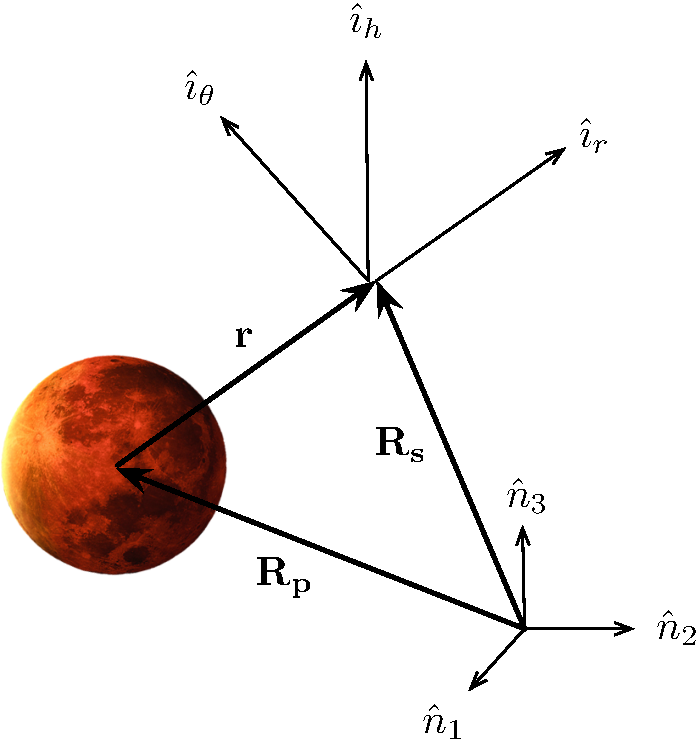
\includegraphics[width=5cm]{Figures/hillPoint}
	}
	\caption{Illustration of the Hill orbit frame $\mathcal{H}$, and the inertial frame $\mathcal{N}$.}
	\label{fig:Fig1}
\end{figure}

\section{Reference Frame Definitions}
A general axis is to be aligned with a principal Hill-frame axis and stay pointing fixedly on it. Note that the presented technique does not require the hill orbit frame $\mathcal{H}:\{ \hat{\bm\imath}_{r}, \hat{\bm\imath}_{\theta}, \hat{\bm\imath}_{h} \}$ to be the inertial frame in use. Figure 1 illustrates the situation assessed.

\section{Angular Velocity Descriptions}
Let the general reference frame associated to this pointing attitude be $\mathcal{R}$. The attitude tracking control requires the angular rate $\bm\omega_{R/N}$ and acceleration $\dot{\bm\omega}_{R/N}$. The angular velocity of the Hill frame is given by
\begin{equation}
	\label{eq:dbeta}
	\bm\omega_{H/N} = \dot f \hat{\bm\imath}_{h} 
\end{equation}
where $\dot f$ is the time-varying true anomaly rate applicable for both cirular and elliptic orbits, and $\hat{\bm\imath}_{h}$ is the orbit's normal direction. Since the pointing towards the orbit axis is constant, the desired reference $\mathcal{R}$ does not move relative to the Hill orbit frame. Thus, the angular velocity of the reference frame happens to be
\begin{equation}
	\label{eq:dbeta}
	\bm\omega_{R/N} = \bm\omega_{R/H} - \bm\omega_{H/N} = \dot{f} \hat{\bm\imath}_{h}
\end{equation}
It is straightforward to compute the acceleration vector of the reference frame
\begin{equation}
	\label{eq:dbeta}
	\dot\omega_{R/N} = \ddot{f} \hat{\bm\imath}_{h}
\end{equation}

\bibliographystyle{unsrt}
\bibliography{references}

\end{document}
